\section{Options Introduction}
\textbf{Options} are a financial derivative that get their price from an underlying asset, such as a stock, bond, or commodity. Options come with a \textit{premium}, a price paid in order to purchase or sell an option.
\\
\\
The two types of option are \textbf{calls} and \textbf{puts}. A \textbf{call option} gives the holder the right but not obligation to buy the underlying asset at a set \textit{strike price}. A \textbf{put option} gives the holder the right but not obligation to sell the underlying asset at a set strike price. 
\\
\\
There are two ways these options can be exercised. A \textbf{European option} can only be exercised at a specific date known as the \textit{maturity date} or \textit{expiration}. \textbf{American options} can be exercised on any date before expiration. For this paper, we will focus on European options.

\subsection{Valuing Options}
Options have \textbf{intrinsic} and \textbf{extrinsic} value. \textit{Intrinsic} value is derived from the underlying asset price and the strike price. 
$$Call \; Option \; Intrinsic \; Value = UAC - CSP$$
$$Put \; Option \; Intrinsic \; Value = PSP - UAC$$
Where \textit{UAC} is the underlying asset current price, \textit{CSP} is the call strike price, and \textit{PSP} is the pull strike price. \\
\textit{Extrinsic value} on the other hand comes from \textit{time value} and \textit{volatility}. Time value refers to the amount of time that an option has to expire with intrinsic value. Volatility refers to the amount by which the underlying asset is expected to change until expiration, with more volatility resulting in a greater chance that the option expires with intrinsic value.\cite{OptionsIntro}


\subsection{Important Features of Options}
There are a few important features that are factored in when developing models to price options. 
\begin{enumerate}
    \item The \textit{strike price} is commonly denoted as \textit{K}
    \item Time till maturity, \textit{T}
    \item The \textbf{Implied Volatility} denoted as $\sigma$. This represents what the market thinks the volatility of the underlying asset will be. 
\end{enumerate}
\subsection{Trading Options}
When you purchase an option, you are considered to be long on the put/call. When you sell an option, you are considered to be short on the put/call. Options are a great way for investors to bet on the underlying asset's movement without ever actually purchasing the asset. This allows them to hedge already existing positions in the underlying or speculate on the movement of the underlying with increased leverage. \cite{OptionsIntro}

\begin{enumerate}
    \item An option is considered \textbf{Out the Money (OTM)} when the profit on the option is negative. 
    \item An option is considered \textbf{At the Money (ATM)} at the profit break-even point. 
    \item An option is considered \textbf{In the Money (ITM)} when the profit on the option is positive
\end{enumerate}


% Below are payoff diagrams to provide a better understanding.
% \begin{figure}[!h]
%     \begin{center}
%         \subfigure[Long Call]{%
%             \label{fig:first}
%             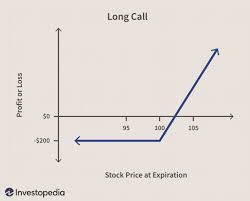
\includegraphics[width=0.4\textwidth]{graphics/LongCall.jpg}
%         }%
%         \subfigure[Short Call]{%
%           \label{fig:second}
%           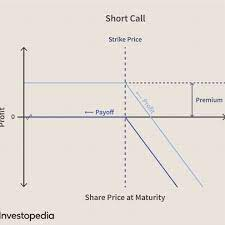
\includegraphics[width=0.4\textwidth]{graphics/ShortCall.jpg}
%         }\\ %  ------- End of the first row ----------------------%
%         \subfigure[Long Put]{%
%             \label{fig:third}
%             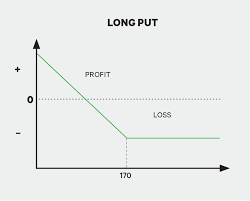
\includegraphics[width=0.4\textwidth]{graphics/LongPut.png}
%         }%
%         \subfigure[Short Put]{%
%             \label{fig:fourth}
%             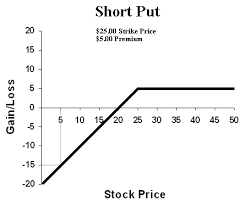
\includegraphics[width=0.4\textwidth]{graphics/ShortPut.png}
%         }%
%     \end{center}
%     \caption{Payoff Diagrams}
%     \label{fig:my_label}
% \end{figure}






\subsection{A Note on Volatility}
While it is impossible to predict the volatility over the duration of an option, we can use a few estimators to find \textbf{historical volatility}.
\\ 
Historical Volatility is defined as the standard deviation of the returns of the underlying multiplied by the square root of the number of time intervals. That is,
$$\sigma^{2}=\frac{1}{N-1}\sum_{n=1}^{N}(x_{i}-\overline{x})^{2}$$
\\
\begin{center}
    $\sigma$ - Volatility \\
    $N$ - Number of observations \\
    $x_{i}$ - Percent return on observation i \\
$\overline{x}$ - Mean return over N observations \\
\end{center}

We can then annualize this by multiplying $\sigma$ by $\sqrt{252}$, the number of trading days in a year.
\\
\\
Another common measure of volatility is \textbf{Yang-Zhang Volatility Model} \cite{YangZhang}. First derived in 2000, the model builds upon the  \textbf{Rogers-Satchell Volatility measure}\cite{RogersSatchell} from 1991 and takes into account opening jumps, drift and estimation error. This measure is often used in real applications since it converges to true historical volatility with much fewer observations than previous methods. \\
\\
As such, it can be thought of as the combination of the close-open volatility (overnight, open-close volatility, and a weighted average of the Rogers-Satchell Volatility
$$\sigma_{Yang-Zhang} = \sqrt{\sigma_o^2+k\sigma_c^2+(1-k)\sigma_{TS}^2}$$
Where 
$$k=\frac{\alpha - 1}{\alpha + \frac{T+1}{T-1}}$$

$$\sigma_o^2 = \frac{1}{T-1}\sum_{t=1}^T \left(\ln{\frac{o_t}{c_{t-1}}} - Avg\ln{\frac{o_t}{c_{t-1}}}\right)^2, overnight \; volatility$$

$$\sigma_c^2 = \frac{1}{T-1}\sum_{t=1}^T \left(\ln{\frac{c_t}{o_{t}}} - Avg\ln{\frac{c_t}{o_{t}}}\right)^2, open-close \; volatility$$

$$\sigma_{RS} = \sqrt{\frac{1}{T}\sum_{t=1}^{T}\ln\left(\frac{h_{t}}{c_{t}}\right)\ln\left(\frac{h_{t}}{o_{t}}\right)+\ln\left(\frac{l_{t}}{c_{t}}\right)\ln\left(\frac{l_{t}}{o_{t}}\right)}, Rogers-Satchell\ Volatility$$
\vspace{.5mm}
$$\alpha = \frac{E[(u(u-c)+d(d-c))^2]}{\sigma^4(1-f)^2}$$
$$T = number \; of \; days \; in \; the \; sample \; period$$
$$o_t = open \; price \; on \; day \; t$$
$$h_t = high \; price \; on \; day \; t$$
$$l_t = low \; price \; on \; day \; t$$
$$c_t = close \; price \; on \; day \; t$$



